\documentclass[12pt, titlepage]{article}

\usepackage{fullpage}
\usepackage[round]{natbib}
\usepackage{multirow}
\usepackage{booktabs}
\usepackage{tabularx}
\usepackage{graphicx}
\usepackage{float}
\usepackage{hyperref}
\usepackage{tikz}
\usetikzlibrary{arrows.meta, positioning}
\hypersetup{
    colorlinks,
    citecolor=blue,
    filecolor=black,
    linkcolor=red,
    urlcolor=blue
}

\input{../../Comments.text}
\input{../../Common.text}

\newcounter{acnum}
\newcommand{\actheacnum}{AC\theacnum}
\newcommand{\acref}[1]{AC\ref{#1}}

\newcounter{ucnum}
\newcommand{\uctheucnum}{UC\theucnum}
\newcommand{\uref}[1]{UC\ref{#1}}

\newcounter{mnum}
\newcommand{\mthemnum}{M\themnum}
\newcommand{\mref}[1]{M\ref{#1}}

\begin{document}

\title{Module Guide for \progname{}\\ \large Design Document Revision $-1$}
\author{\authname}
\date{\today}

\maketitle

\pagenumbering{roman}

\section{Revision History}

\begin{tabularx}{\textwidth}{p{3cm} p{3cm} X}
\toprule
\textbf{Date} & \textbf{Version} & \textbf{Notes}\\
\midrule
Nov 16, 2026 & Rev $-1$ & First module guide for the proof of concept: module decomposition, anticipated and unlikely changes, and traceability. Semantics are deferred to Rev 0.\\
\bottomrule
\end{tabularx}

\newpage

\section{Reference Material}

This section records information for easy reference.

\subsection{Abbreviations and Acronyms}

See the SRS \citep{TandemSRS}, available at
\href{https://github.com/tandemkv/Tandem/blob/main/pdfs/SRS-Volere/SRS.pdf}{pdfs/SRS-Volere/SRS.pdf},
for a complete list of symbols, abbreviations and acronyms. The additional terms
used in this document are AC (anticipated change), UC (unlikely change), M
(module) and MG (Module Guide).

\newpage

\tableofcontents

\listoftables

\listoffigures

\newpage

\pagenumbering{arabic}

\section{Introduction}

\progname{} is a proof of concept for reusing the key--value cache of one
language model when a conversation moves to another model. Without reuse, the
receiving model re-reads the whole conversation (prefill) before it can answer.
With reuse, a cache predicted from the source model is loaded into the target
model, and only the new text is prefilled. The requirements are in the SRS.
The source requirements are referenced by ID (for example FR-05, SR-02).

The modules below follow the principle of information hiding
\citep{ParnasEtAl1984}. Each module hides one design decision.

\section{Anticipated and Unlikely Changes} \label{SecChange}

This section lists possible changes to the system. Anticipated changes are
listed in Section \ref{SecAchange}, and unlikely changes in Section \ref{SecUchange}.

\subsection{Anticipated Changes} \label{SecAchange}

Anticipated changes are the source of the information that is to be hidden
inside the modules. Changing one of them should only require changing the one
module that hides the associated decision.

\begin{description}
\item[\refstepcounter{acnum} \actheacnum \label{acPair}:] The source and target
  model pair, and the checkpoints used for each (SRS LC1).
\item[\refstepcounter{acnum} \actheacnum \label{acRuntime}:] The inference
  library and its revision pinning (for example Transformers versus another
  serving engine) (SRS LC2).
\item[\refstepcounter{acnum} \actheacnum \label{acCacheRep}:] The in-memory
  representation of a KV cache and its provenance tags (SRS LC2).
\item[\refstepcounter{acnum} \actheacnum \label{acMapping}:] The translators:
  the method that maps source KV features to target KV features (such as ridge
  regression, an affine map or an attention network), the token pairing and
  positional conversion it relies on, the directions each supports, the
  checkpoint for each direction, and how checkpoints are fitted (SRS OI1).
\item[\refstepcounter{acnum} \actheacnum \label{acPolicy}:] The routing: the
  classifier that scores a request, and the label-to-model table and complexity
  threshold (SRS LC4).
\item[\refstepcounter{acnum} \actheacnum \label{acApprove}:] The setups approved
  for reuse, their preapproval thresholds, and the evidence each needs before
  approval (SRS LC4).
\item[\refstepcounter{acnum} \actheacnum \label{acLog}:] The fields recorded for
  each request (SRS LC3).
\item[\refstepcounter{acnum} \actheacnum \label{acWorkload}:] The workloads
  used for comparisons (SRS LC3).
\item[\refstepcounter{acnum} \actheacnum \label{acHardware}:] The hardware on
  which models run (SRS LC3).
\item[\refstepcounter{acnum} \actheacnum \label{acLimits}:] The numeric limits
  for quality loss, canary checks, fallback admission, cache memory and expiry,
  and the comparison tolerances, each with its version and reason (SRS LC4;
  HA SR-09 to SR-14).
\item[\refstepcounter{acnum} \actheacnum \label{acJudge}:] The scoring rules:
  the answer-equivalence judge and its threshold, and the task-score metric used
  by the quality gate (answer F1, the equivalence judge, or both).
\item[\refstepcounter{acnum} \actheacnum \label{acHandoff}:] The boundary of the
  prefix that is translated: the whole history or only the part before the
  question, with the receiver prefilling the rest.
\end{description}

\subsection{Unlikely Changes} \label{SecUchange}

These decisions are fixed at architecture time. A change would affect many
modules, so they are not expected to change.

\begin{description}
\item[\refstepcounter{ucnum} \uctheucnum \label{ucTraining}:] Base language
  models are not trained by the system; training and routing of base models
  stay external (SRS UC1).
\item[\refstepcounter{ucnum} \uctheucnum \label{ucSingle}:] Execution runs on
  one server (SRS UC2).
\item[\refstepcounter{ucnum} \uctheucnum \label{ucExact}:] Reuse requires an
  exact shared prefix and permission checks, not semantic similarity (SRS UC3).
\end{description}

\section{Module Hierarchy} \label{SecMH}

The hierarchy is decomposed by secrets. Leaf modules are implemented. Non-leaf
modules are for organisation only.

\begin{description}
\item [\refstepcounter{mnum} \mthemnum \label{mAccel}:] Accelerator Interface
\item [\refstepcounter{mnum} \mthemnum \label{mConv}:] Conversation Management
\item [\refstepcounter{mnum} \mthemnum \label{mCtrl}:] Request Control
\item [\refstepcounter{mnum} \mthemnum \label{mBench}:] Comparison Benchmark
\item [\refstepcounter{mnum} \mthemnum \label{mSelect}:] Model Selection
\item [\refstepcounter{mnum} \mthemnum \label{mReuse}:] Reuse Policy
\item [\refstepcounter{mnum} \mthemnum \label{mHandoff}:] Cache Handoff
\item [\refstepcounter{mnum} \mthemnum \label{mCompat}:] Cache Compatibility
\item [\refstepcounter{mnum} \mthemnum \label{mLife}:] Request Lifecycle
\item [\refstepcounter{mnum} \mthemnum \label{mLog}:] Run Logging
\item [\refstepcounter{mnum} \mthemnum \label{mQuality}:] Quality Measurement
\item [\refstepcounter{mnum} \mthemnum \label{mModelRun}:] Model Runtime
\item [\refstepcounter{mnum} \mthemnum \label{mCache}:] Cache Store
\item [\refstepcounter{mnum} \mthemnum \label{mMap}:] Cache Mapper
\item [\refstepcounter{mnum} \mthemnum \label{mFit}:] Predictor Fitting
\item [\refstepcounter{mnum} \mthemnum \label{mLimits}:] Limits
\end{description}

\begin{table}[h!]
\centering
\begin{tabular}{p{0.3\textwidth} p{0.6\textwidth}}
\toprule
\textbf{Level 1} & \textbf{Level 2}\\
\midrule

{Hardware-Hiding Module} & Accelerator Interface \mref{mAccel}\\
\midrule

\multirow{10}{0.3\textwidth}{Behaviour-Hiding Module} & Conversation Management \mref{mConv}\\
& Request Control \mref{mCtrl}\\
& Comparison Benchmark \mref{mBench}\\
& Model Selection \mref{mSelect}\\
& Reuse Policy \mref{mReuse}\\
& Cache Handoff \mref{mHandoff}\\
& Cache Compatibility \mref{mCompat}\\
& Request Lifecycle \mref{mLife}\\
& Run Logging \mref{mLog}\\
& Quality Measurement \mref{mQuality}\\
\midrule

\multirow{5}{0.3\textwidth}{Software Decision Module} & Model Runtime \mref{mModelRun}\\
& Cache Store \mref{mCache}\\
& Cache Mapper \mref{mMap}\\
& Predictor Fitting \mref{mFit}\\
& Limits \mref{mLimits}\\
\bottomrule

\end{tabular}
\caption{Module Hierarchy}
\label{TblMH}
\end{table}

\section{Connection Between Requirements and Design} \label{SecConnection}

The design satisfies the SRS requirements as follows. The decisions made
between the requirements and the design are recorded here:

\begin{itemize}
\item Reuse is only attempted when Reuse Policy approves the setup and Cache
  Compatibility accepts the candidate cache (FR-13, FR-14, SR-02). Otherwise
  the request is processed natively (FR-06). The fallback is therefore a
  deliberate path, not an error path.
\item Cross-model reuse requires a Cache Mapper for the chosen pair. Without
  one, the request fails with an explicit error or is processed natively. It is
  never silently answered with a stale or mismatched cache (FR-07, SR-02).
\item The run-time canary check (SR-10) is part of Cache Compatibility
  (\mref{mCompat}), next to the static checks: both decide whether a cache may be
  used. Cache Handoff runs it before a predicted cache is loaded.
\item Fallback admission, the queue limit and the automatic shutoff of
  cross-model reuse (SR-13) are part of Request Lifecycle (\mref{mLife}), which
  already admits, tracks and releases each request.
\item Approval of a setup from its test evidence (SR-09, FR-14) is part of Reuse
  Policy (\mref{mReuse}), which owns the list of approved setups.
\item Checksums and source records for caches (SR-11) are checked by Cache
  Compatibility (\mref{mCompat}) as one of its rules, separate from the storage
  layout in Cache Store, because the integrity format and the layout are
  decided for different reasons.
\end{itemize}

\noindent The following decisions are open. The design above assumes the
options listed; each must be confirmed by the team before Rev 0:
\begin{itemize}
\item \textbf{NFR-05 for cross-model setups.} NFR-05 requires identical greedy
  output and logits within tolerance for every approved setup. Cross-model
  prediction is approximate (HA H8), so the design assumes that cross-model
  setups are approved by the quality gate (SR-09) and that NFR-05 keeps its
  exact check for same-model reuse only.
\item \textbf{The metric for SR-09.} The design assumes the task-score metric is
  set by \acref{acJudge}; the candidates are answer F1, the equivalence judge,
  or both.
\item \textbf{Placement of T-QUAL-2.} The design assumes the cross-model
  translation check is a component-level evaluation, reported in the ML Model
  Report, not a system test in the VnV Plan.
\end{itemize}

\section{Module Decomposition} \label{SecMD}

Each module has a \emph{Secrets} field, a brief statement of the design decision
the module hides, and a \emph{Services} field, what the module does without
saying how.

All leaf modules are implemented by \progname{}. External libraries are used
inside modules, not as modules: Accelerator Interface wraps PyTorch's device
layer, and Model Runtime wraps Hugging Face Transformers.

\subsection{Hardware-Hiding Modules}

\begin{description}
\item[Secrets:] The data structures and algorithms used to implement the virtual
  hardware.
\item[Services:] Serves as virtual hardware used by the rest of the system. The
  modules provide the interface between the hardware and the software.
\end{description}

\subsubsection{Accelerator Interface (\mref{mAccel})}

\begin{description}
\item[Secrets:] The physical devices the system runs on (\acref{acHardware}).
\item[Services:] Provides a device handle and a number format for running
  models.
\item[Type of Module:] Library
\end{description}

\subsection{Behaviour-Hiding Modules}

\begin{description}
\item[Secrets:] The contents of the required behaviours.
\item[Services:] Provides externally visible behaviour specified in the SRS. The
  modules communicate with the software decision modules.
\end{description}

\subsubsection{Conversation Management (\mref{mConv})}

\begin{description}
\item[Secrets:] The representation of a conversation across turns.
\item[Services:] Sends a user message through Request Control. Updates the
  conversation only after a successful answer. A failure leaves the previous
  state unchanged (FR-03, SR-04).
\item[Type of Module:] Abstract Data Type
\end{description}

\subsubsection{Request Control (\mref{mCtrl})}

\begin{description}
\item[Secrets:] The procedure for handling one request from validation to delivery.
\item[Services:] Processes one request from validation to delivery. Rejects a
  malformed or out-of-range request with a stable error code before any model
  work (FR-01, NFR-12). Selects the model, decides whether to reuse a cache, runs
  the request, and records it. Before reusing a same-model cache, it checks the
  cache with Cache Compatibility (\mref{mCompat}) (FR-04). When reuse is not used, it runs the whole prompt
  on the chosen model (FR-06). It returns the output in order, under the correct
  request ID (FR-08). This is the control module, at the top of the use
  hierarchy below Conversation Management.
\item[Type of Module:] Library
\end{description}

\subsubsection{Comparison Benchmark (\mref{mBench})}

\begin{description}
\item[Secrets:] The procedure for comparing reuse with native processing on the same workloads (\acref{acWorkload}).
\item[Services:] Runs the same workload with and without reuse, using the same
  prompts and the same token boundaries, and produces a report (FR-11, FR-12).
\item[Type of Module:] Library
\end{description}

\subsubsection{Model Selection (\mref{mSelect})}

\begin{description}
\item[Secrets:] The rule that chooses the answer model for a prompt (\acref{acPolicy}).
\item[Services:] Classifies a request and returns the answer model for it
  (FR-02, NFR-09).
\item[Type of Module:] Abstract Object
\end{description}

\subsubsection{Reuse Policy (\mref{mReuse})}

\begin{description}
\item[Secrets:] The criteria a setup must meet before reuse is approved (\acref{acApprove}).
\item[Services:] Approves a setup from its recorded evidence: the held-out
  quality result, the output and privacy tests, and the failure-handling tests.
  A missing or failed record means the setup is not approved (FR-14, SR-09,
  NFR-05). Decides whether reuse may be attempted for a request; the decision
  depends only on the approved setups and on the request's permission and
  history (FR-13, NFR-08, SR-01, SR-05, SR-12). The supported directions come
  from Cache Mapper (\mref{mMap}).
\item[Type of Module:] Abstract Object
\end{description}

\subsubsection{Cache Handoff (\mref{mHandoff})}

\begin{description}
\item[Secrets:] The way a predicted cache is passed to the target model (\acref{acHandoff}).
\item[Services:] Produces an answer from a predicted cache, with the suffix
  processed once and in order (FR-05). It seals each predicted cache with Cache
  Compatibility (\mref{mCompat}) as soon as Cache Mapper returns it (SR-11), and
  loads the cache only after the canary check in Cache Compatibility accepts it
  (SR-10). It registers each predicted cache with Request Lifecycle
  (\mref{mLife}), so that unused ones expire (SR-14).
\item[Type of Module:] Library
\end{description}

\subsubsection{Cache Compatibility (\mref{mCompat})}

\begin{description}
\item[Secrets:] The rules that decide whether a cache may be used.
\item[Services:] Accepts a candidate cache or rejects it with a reason (FR-04,
  SR-02, SR-04). Creates the integrity record for a cache and checks it before
  the cache is used (SR-11). Accepts or rejects a predicted cache before it is
  loaded, using a bounded recomputation of its final tokens; this detects badly
  wrong predictions but does not prove a cache correct (SR-10, FR-16).
\item[Type of Module:] Library
\end{description}

\subsubsection{Request Lifecycle (\mref{mLife})}

\begin{description}
\item[Secrets:] The policy that governs a request from admission to release.
\item[Services:] Cancels or times out a request, releases its cache, and
  reports the final state (FR-09, FR-15, SR-03, NFR-06). Admits or queues a
  fallback prefill, rejects requests beyond the queue limit with a retry status,
  and turns cross-model reuse off when the fallback rate is too high, reporting
  the shutoff to the operator (SR-13, NFR-08). Expires unused predicted caches
  within the memory cap and lifetime set in Limits (SR-14).
\item[Type of Module:] Abstract Object
\end{description}

\subsubsection{Run Logging (\mref{mLog})}

\begin{description}
\item[Secrets:] The format of the run log (\acref{acLog}).
\item[Services:] Records each request's status, reuse decision and measurements
  (FR-10, SR-06, NFR-10). Each record includes the translation metadata:
  translator name, checkpoint identity, and whether translation ran.
\item[Type of Module:] Library
\end{description}

\subsubsection{Quality Measurement (\mref{mQuality})}

\begin{description}
\item[Secrets:] The method for judging whether a reused answer matches the native one (\acref{acJudge}).
\item[Services:] Scores an answer against the native answer and the gold
  answer (NFR-03, NFR-05). Computes the task score used by the quality gate in
  Reuse Policy (\mref{mReuse}) (SR-09).
\item[Type of Module:] Library
\end{description}

\subsection{Software Decision Modules}

\begin{description}
\item[Secrets:] The design decision based on mathematical theorems, physical
  facts, or programming considerations. These are not described in the SRS.
\item[Services:] Data structures and algorithms that do not interact with the
  user directly.
\end{description}

\subsubsection{Model Runtime (\mref{mModelRun})}

\begin{description}
\item[Secrets:] The inference library used to run the models (\acref{acPair}, \acref{acRuntime}).
\item[Services:] Implements the answer-model contract (\texttt{AnswerModel}):
  runs a prompt or a list of token IDs with an optional cache, and returns the
  resulting cache.
\item[Type of Module:] Abstract Object
\end{description}

\subsubsection{Cache Store (\mref{mCache})}

\begin{description}
\item[Secrets:] The in-memory representation of a KV cache (\acref{acCacheRep}).
\item[Services:] Creates a tagged cache, reports its length and provenance, and
  copies it (FR-04).
\item[Type of Module:] Abstract Data Type
\end{description}

\subsubsection{Cache Mapper (\mref{mMap})}

\begin{description}
\item[Secrets:] The method that translates one model's cache into another model's cache (\acref{acMapping}).
\item[Services:] Implements the \texttt{KVCacheMapper} contract. Returns a target
  cache and the exact uncached target token IDs, and raises an explicit error
  for an unsupported direction before it changes any state (FR-05, FR-16,
  NFR-05). Returns the checkpoint for a direction, or an explicit error for an
  unsupported or unavailable direction; it never substitutes another
  translator (FR-13). It tokenizes the shared text with each model's tokenizer
  through Model Runtime (\mref{mModelRun}).
\item[Type of Module:] Abstract Object
\end{description}

\subsubsection{Predictor Fitting (\mref{mFit})}

\begin{description}
\item[Secrets:] The procedure that fits a translator from paired caches (\acref{acMapping}).
\item[Services:] Produces a checkpoint and its manifest from paired data, and
  refuses a split whose groups overlap (FR-14, FR-16). It runs offline, not
  during reuse, and builds the paired caches with Model Runtime and Cache Store.
\item[Type of Module:] Library
\end{description}

\subsubsection{Limits (\mref{mLimits})}

\begin{description}
\item[Secrets:] The numeric thresholds used across the design (\acref{acLimits}).
\item[Services:] Provides each limit to the module that enforces it. A change to
  any limit is made here only (NFR-09, SR-09 to SR-14).
\item[Type of Module:] Library
\end{description}

\section{Traceability Matrix} \label{SecTM}

This section shows two traceability matrices: between the modules and the
requirements, and between the modules and the anticipated changes.

\begin{table}[H]
\centering
\small
\begin{tabular}{p{0.2\textwidth} p{0.7\textwidth}}
\toprule
\textbf{Req.} & \textbf{Modules}\\
\midrule
FR-01 & \mref{mCtrl}\\
FR-02 & \mref{mSelect}, \mref{mModelRun}\\
FR-03 & \mref{mConv}, \mref{mCompat}\\
FR-04 & \mref{mCtrl}, \mref{mCompat}, \mref{mCache}\\
FR-05 & \mref{mHandoff}, \mref{mMap}, \mref{mAccel}\\
FR-06 & \mref{mCtrl}, \mref{mModelRun}\\
FR-07 & \mref{mCtrl}, \mref{mLife}\\
FR-08 & \mref{mCtrl}\\
FR-09 & \mref{mLife}\\
FR-10 & \mref{mLog}\\
FR-11 & \mref{mBench}\\
FR-12 & \mref{mBench}\\
FR-13 & \mref{mReuse}, \mref{mMap}\\
FR-14 & \mref{mReuse}, \mref{mBench}, \mref{mFit}\\
FR-15 & \mref{mLife}\\
FR-16 & \mref{mMap}, \mref{mCompat}, \mref{mFit}\\
NFR-01 & \mref{mLog}, \mref{mBench}\\
NFR-02 & Not a module: setup instructions are a documentation deliverable\\
NFR-03 & \mref{mQuality}\\
NFR-04 & \mref{mBench}, \mref{mAccel}\\
NFR-05 & \mref{mQuality}, \mref{mMap}, \mref{mModelRun}, \mref{mReuse}\\
NFR-06 & \mref{mLife}, \mref{mCtrl}\\
NFR-07 & \mref{mCtrl}, \mref{mBench}\\
NFR-08 & \mref{mReuse}, \mref{mBench}, \mref{mLife}\\
NFR-09 & \mref{mSelect}, \mref{mReuse}, \mref{mLimits}\\
NFR-10 & \mref{mBench}, \mref{mLog}\\
NFR-12 & \mref{mCtrl}, \mref{mLog}\\
SR-01 & \mref{mReuse}, \mref{mConv}\\
SR-02 & \mref{mCompat}\\
SR-03 & \mref{mLife}, \mref{mCache}\\
SR-04 & \mref{mConv}, \mref{mCompat}\\
SR-05 & \mref{mReuse}, \mref{mCompat}\\
SR-06 & \mref{mLog}\\
SR-09 & \mref{mReuse}, \mref{mQuality}, \mref{mLimits}\\
SR-10 & \mref{mCompat}, \mref{mHandoff}, \mref{mLimits}\\
SR-11 & \mref{mCompat}, \mref{mHandoff}\\
SR-12 & \mref{mReuse}\\
SR-13 & \mref{mLife}, \mref{mCtrl}, \mref{mLimits}\\
SR-14 & \mref{mHandoff}, \mref{mLife}, \mref{mLimits}\\
DR-01 & Not a module: installation and operation guide is a documentation deliverable\\
DR-02 & \mref{mBench}, \mref{mQuality}; the written explanation is a documentation deliverable\\
\bottomrule
\end{tabular}
\caption{Trace Between Requirements and Modules}
\label{TblRT}
\end{table}

\noindent NFR-02, DR-01 and DR-02 are not design requirements. They ask for
setup instructions and written explanations, which are documentation
deliverables, so no module satisfies them directly. The SR-09 to SR-14 rows
come from the Hazard Analysis.

\begin{table}[H]
\centering
\begin{tabular}{p{0.2\textwidth} p{0.7\textwidth}}
\toprule
\textbf{AC} & \textbf{Modules}\\
\midrule
\acref{acPair} & \mref{mModelRun}\\
\acref{acRuntime} & \mref{mModelRun}\\
\acref{acCacheRep} & \mref{mCache}\\
\acref{acMapping} & \mref{mMap}, \mref{mFit}\\
\acref{acPolicy} & \mref{mSelect}\\
\acref{acApprove} & \mref{mReuse}\\
\acref{acLog} & \mref{mLog}\\
\acref{acWorkload} & \mref{mBench}\\
\acref{acHardware} & \mref{mAccel}\\
\acref{acLimits} & \mref{mLimits}\\
\acref{acJudge} & \mref{mQuality}\\
\acref{acHandoff} & \mref{mHandoff}\\
\bottomrule
\end{tabular}
\caption{Trace Between Anticipated Changes and Modules}
\label{TblACT}
\end{table}

Each anticipated change is hidden by exactly one module, and each module has one
secret, with five exceptions:

\begin{enumerate}
\item \textbf{One module hides two changes.} Model Runtime (\mref{mModelRun})
  hides both the model pair (\acref{acPair}) and the inference library
  (\acref{acRuntime}). They come from different SRS changes (LC1 and LC2), but
  both decide how a model is loaded and run, so splitting them would put one
  decision in two places.
\item \textbf{One change is hidden by two modules.} The translators
  (\acref{acMapping}) are shared by Cache Mapper (\mref{mMap}), which applies a
  translator at run time, and Predictor Fitting (\mref{mFit}), which fits it
  offline. They are kept separate because Predictor Fitting runs as a separate
  offline program with dependencies (training data and an optimiser) that the
  serving path must not load. The checkpoint file is their only shared
  interface: Predictor Fitting writes it and Cache Mapper reads it.
\item \textbf{Four modules hide no anticipated change.} Conversation Management
  (\mref{mConv}), Request Control (\mref{mCtrl}), Cache Compatibility
  (\mref{mCompat}) and Request Lifecycle (\mref{mLife}) are behaviour-hiding
  modules whose secret is the required behaviour itself (FR-01, FR-03, FR-04,
  FR-06 to FR-09, FR-15, SR-02, SR-10, SR-11, SR-13, SR-14). They change only
  if the SRS changes.
\item \textbf{Cache Compatibility (\mref{mCompat}) holds both the static checks
  and the canary test.} Both answer one question, whether a cache may be used,
  and both return the same verdict and rejection reasons. Splitting them would
  give two modules that each decide acceptance.
\item \textbf{Request Lifecycle (\mref{mLife}) holds request states, fallback
  admission and the expiry of predicted caches.} All three act on the same set of
  in-flight requests and the same memory. Splitting them would duplicate that
  state across modules.
\end{enumerate}

\section{Use Hierarchy Between Modules} \label{SecUse}

A module \emph{uses} another if the first module's correct behaviour depends on
the second being correct \citep{Parnas1978}. The arrows point from the user to
the module used. The hierarchy is a directed acyclic graph, with the control
modules at the top.

\begin{figure}[H]
\centering
\resizebox{\textwidth}{!}{%
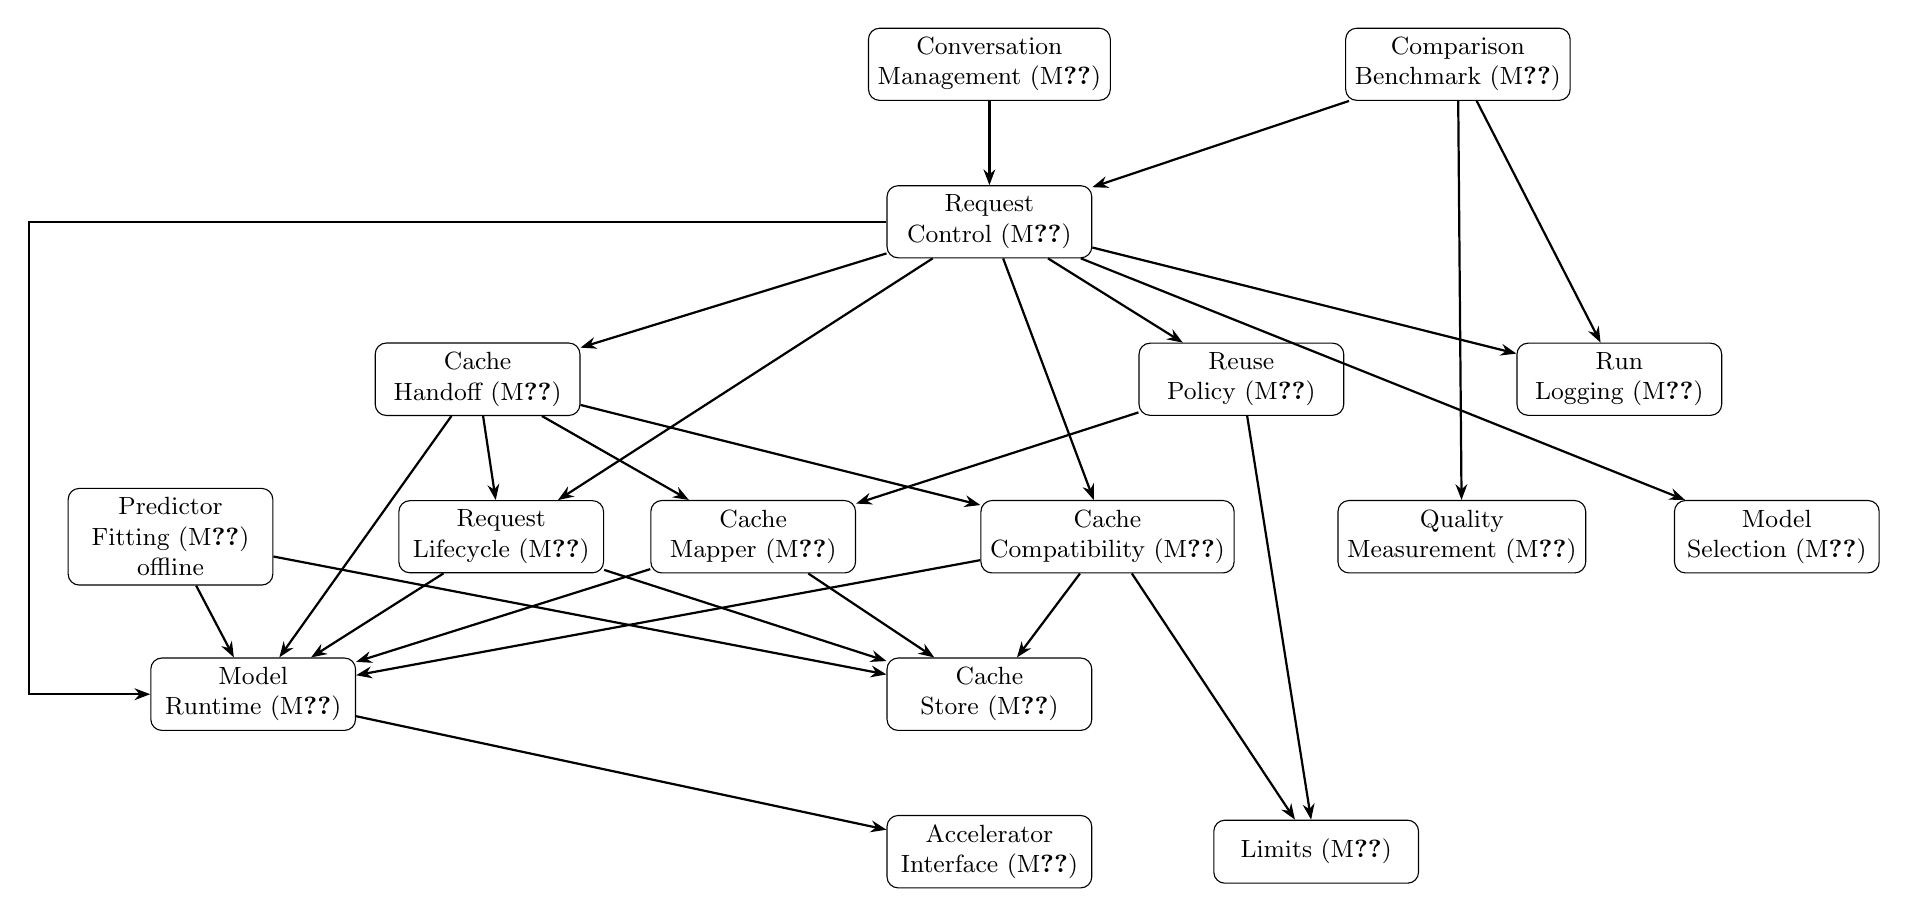
\begin{tikzpicture}[
  mod/.style={draw, rounded corners, align=center, minimum width=2.6cm, minimum height=0.8cm, font=\small},
  arr/.style={-{Stealth[length=2mm]}, thick}]
  % Row A: entry points
  \node[mod] (conv) at (0,8) {Conversation\\Management (\mref{mConv})};
  \node[mod] (bench) at (5.95,8) {Comparison\\Benchmark (\mref{mBench})};
  % Row B: control
  \node[mod] (ctrl) at (0,6) {Request\\Control (\mref{mCtrl})};
  % Row C: request steps
  \node[mod] (handoff) at (-6.5,4) {Cache\\Handoff (\mref{mHandoff})};
  \node[mod] (reuse) at (3.2,4) {Reuse\\Policy (\mref{mReuse})};
  \node[mod] (log) at (8,4) {Run\\Logging (\mref{mLog})};
  % Row D: lifecycle, translation, cache checks, scoring, selection and offline fitting
  \node[mod] (fit) at (-10.4,2) {Predictor\\Fitting (\mref{mFit})\\offline};
  \node[mod] (life) at (-6.2,2) {Request\\Lifecycle (\mref{mLife})};
  \node[mod] (map) at (-3.0,2) {Cache\\Mapper (\mref{mMap})};
  \node[mod] (compat) at (1.5,2) {Cache\\Compatibility (\mref{mCompat})};
  \node[mod] (quality) at (6,2) {Quality\\Measurement (\mref{mQuality})};
  \node[mod] (select) at (10,2) {Model\\Selection (\mref{mSelect})};
  % Row E: software decisions
  \node[mod] (model) at (-9.35,0) {Model\\Runtime (\mref{mModelRun})};
  \node[mod] (cache) at (0,0) {Cache\\Store (\mref{mCache})};
  % Row F: hardware and limits
  \node[mod] (accel) at (0,-2) {Accelerator\\Interface (\mref{mAccel})};
  \node[mod] (limits) at (4.15,-2) {Limits (\mref{mLimits})};
  % Arrows (user -> used)
  \draw[arr] (conv) -- (ctrl);
  \draw[arr] (bench) -- (ctrl);
  \draw[arr] (bench) -- (log);
  \draw[arr] (bench) -- (quality);
  \draw[arr] (ctrl) -- (handoff);
  \draw[arr] (ctrl) -- (life);
  \draw[arr] (ctrl) -- (log);
  \draw[arr] (ctrl) -- (reuse);
  \draw[arr] (ctrl) -- (select);
  \draw[arr] (ctrl) -- (compat);
  \draw[arr] (ctrl.west) -- (-12.2,6) |- (model.west);
  \draw[arr] (handoff) -- (life);
  \draw[arr] (handoff) -- (map);
  \draw[arr] (handoff) -- (compat);
  \draw[arr] (handoff) -- (model);
  \draw[arr] (life) -- (model);
  \draw[arr] (life) -- (cache);
  \draw[arr] (reuse) -- (map);
  \draw[arr] (reuse) -- (limits);
  \draw[arr] (fit) -- (model);
  \draw[arr] (fit) -- (cache);
  \draw[arr] (map) -- (model);
  \draw[arr] (map) -- (cache);
  \draw[arr] (compat) -- (model);
  \draw[arr] (compat) -- (cache);
  \draw[arr] (compat) -- (limits);
  \draw[arr] (model) -- (accel);
\end{tikzpicture}}
\caption{Use hierarchy among modules (numbers match the module list). Predictor
Fitting (\mref{mFit}) runs offline, and no module uses it. The arrow from Request
Lifecycle (\mref{mLife}) to Limits (\mref{mLimits}) is not drawn, to keep the
figure readable.}
\label{FigUH}
\end{figure}

\section{User Interfaces}

The proof of concept has no graphical user interface; it is run from Python
scripts.

\section{Design of Communication Protocols}

Not applicable. The system runs in one process on one server (\uref{ucSingle}),
and modules communicate by function calls.

\section{Database Design}

Not applicable. The system has no database; checkpoints, datasets and logs are
files.

\section{Timeline}

Deferred to Rev 0.

\section*{Appendix --- Generative AI Use Disclosure}

\subsection*{AI Tools Used}

\begin{itemize}
\item Claude Code, a command-line tool, using the model Claude Opus 5.5
  (model ID \texttt{claude-opus-5-5}).
\end{itemize}
No other AI tools were used in drafting this document.

\subsection*{How and Where Used}

\begin{itemize}
\item \textbf{Reviewing the document.} The draft was checked against the course
  MG checklist, the template and the Rev $-1$ rubric. The tool listed modules
  with more than one secret, wrong module types, uses that pointed upward or
  disagreed with the code, and anticipated changes that were not hidden by
  exactly one module.
\item \textbf{Modifying text.} The tool removed sections that Rev $-1$ does not
  require, merged eleven modules into others (27 to 16 modules), reduced the
  anticipated changes to the SRS likely changes plus two design decisions, and rewrote
  secrets, anticipated changes, traceability rows and the use hierarchy
  to match.
\item \textbf{Modifying diagrams.} The tool redrew the use hierarchy so that
  every arrow points down.
\end{itemize}

\subsection*{Verification of AI-Generated Content}

\begin{itemize}
\item Every change was proposed as a plan and approved by a team member before
  it was made.
\item Argument names and uses were checked against the source code in
  \texttt{src/}, and requirement IDs against the SRS and the Hazard Analysis.
\item The document was rebuilt with no LaTeX errors or undefined references, and
  the use hierarchy was checked by rendering it.
\end{itemize}
The team reviewed the final text and is responsible for its accuracy.

%\section*{References}

\bibliographystyle{plainnat}
\bibliography{../../../refs/References}

\end{document}
